%! suppress = GroupedSubSupScript
%! suppress = Ellipsis
% Define document class
%\documentclass[twocolumn,twocolappendix,linenumbers]{aastex631}
\documentclass[modern,linenumbers]{aastex631}
% Some entries inspired from a preamble by Adrian Price-Whelan, https://github.com/adrn/PhaseSpiralAsteroseismology/blob/main/tex/preamble.tex

\usepackage{showyourwork}

% Latex imports
\let\tablenum\relax             % necessary for AASTeX
\usepackage{siunitx}
\sisetup{range-phrase= \text{--}, range-units=single, separate-uncertainty=true}
\sisetup{separate-uncertainty=true}
\usepackage{blindtext}          % Filler text
\usepackage{xcolor}
\usepackage[T1]{fontenc}

\usepackage[toc,nogroupskip,nohypertypes={glossary}]{glossaries} % import after hyperref
\glsdisablehyper

\newglossaryentry{HST}{name={HST}, description={Hubble Space Telescope}, first={Hubble Space Telescope (HST)}}
\newglossaryentry{NIR}{name={NIR}, description={Near-Infrared}, first={near-infrared (NIR)}}
\newglossaryentry{MIR}{name={MIR}, description={Mid-Infrared}, first={mid-infrared (MIR)}}
\newglossaryentry{FIR}{name={FIR}, description={Far-Infrared}, first={far-infrared (FIR)}}
\newglossaryentry{FUV}{name={FUV}, description={Far-Ultraviolet}, first={far-Ultraviolet (FUV)}}
\newglossaryentry{NUV}{name={NUV}, description={Near-Ultraviolet}, first={near-Ultraviolet (NUV)}}
\newglossaryentry{EUV}{name={EUV}, description={extreme-Ultraviolet}, first={extreme-Ultraviolet (EUV)}}
\newglossaryentry{SED}{name={SED}, description={Spectral energy distribution}, first={spectral energy distribution (SED)}, firstplural={spectral energy distributions (SEDs)}}
\newglossaryentry{ppm}{name={ppm}, description={parts per million}, first={parts per million (ppm)}}
\newglossaryentry{PDF}{name={PDF}, description={Probability density function}, first={probability density function (PDF)}, firstplural={probability density functions (PDF)}}
\newglossaryentry{PLATO}{name={PLATO}, description={PLAnetary Transits and Oscillations of stars}, first={PLATO~\citep[][]{Rauer2014}}}
\newglossaryentry{PSF}{name={PSF},description={Point Spread Function}, first={point spread function (PSF)}, firstplural={point spread functions (PSF)}}
\newglossaryentry{SFD}{name={SFD}, description={Size frequency distribution}, first={size frequency distribution (SFD)}, firstplural={Size frequency distributions (SFD)}}
\newglossaryentry{SNR}{name={SNR}, description={Signal-to-noise ratio}, first={signal-to-noise ratio (SNR)}}
\newglossaryentry{RV}{name={RV}, description={Radial Velocity}, first={Radial Velocity (RV)}, firstplural={Radial Velocities (RV)}}
\newglossaryentry{TTV}{name={TTV}, description={Transit Timing Variation}, first={transit timing variation (TTV)}, firstplural={transit timing variations (TTVs)}}
\newglossaryentry{TESS}{name={TESS}, description={Transiting Exoplanet Survey Satellite}, first={Transiting Exoplanet Survey Satellite~\citep[\textit{TESS},][]{Ricker2014}}}
\newglossaryentry{TIC}{name={TIC}, description={\textit{TESS} Input Catalog}, first={\textit{TESS} Input Catalog~\citep[TIC,][]{Stassun2018}}}
\newglossaryentry{JWST}{name={JWST}, description={James Webb Space Telescope}, first={James Webb Space Telescope~\citep[\textit{JWST},][]{Beichman2014}}}
\newglossaryentry{HZ}{name={HZ}, description={habitable zone}, first={habitable zone (HZ)}}
\newglossaryentry{EEC}{name={EEC}, description={exo-Earth candidate}, first={exo-Earth candidate (EEC)}, firstplural={exo-Earth candidates (EEC)}}
%\newglossaryentry{}{name={}, description={}, first={}, firstplural={}}


% package to open file containing variables
\usepackage{datatool, filecontents}
\DTLsetseparator{,}% Set the separator between the columns.

% import data
\DTLloaddb[noheader, keys={thekey,thevalue}]{variables}{variables.dat}
% Loads variables.dat with column headers 'thekey' and 'thevalue'
\newcommand{\var}[1]{\ensuremath{\DTLfetch{variables}{thekey}{#1}{thevalue}}}

% paper comments
\usepackage{comment}						 % comments that can be switched visible/invisible
\includecomment{comment}
%\specialcomment{outtake}{\begingroup\sffamily\color{gray}}{\endgroup}
%\specialcomment{note}{\begingroup\sffamily\color{red!40!green!70!blue!90}}{\endgroup}
\specialcomment{note}{\begingroup\sffamily\color{gray}}{\endgroup}
%\excludecomment{note}                       % switch notes off

%% switch TODO notes on/off
\usepackage[backgroundcolor=red!20!green!40!blue!10, textsize=tiny]{todonotes}
% \usepackage[disable]{todonotes}			% switches all todo notes to invisible
\usepackage{regexpatch}
\makeatletter
\xpatchcmd{\@todo}{\setkeys{todonotes}{#1}}{\setkeys{todonotes}{inline,#1}}{}{}
\makeatother

%% manuscript revision
%\newcommand{\rev}[1]{{\textbf{#1}}}    % on
\newcommand{\rev}[1]{{#1}}              % off

%% ... and second revision
\newcommand{\revv}[1]{{\textbf{#1}}}    % on
%\newcommand{\revv}[1]{{#1}}            % off

% ---------------------------------
% PAPER VARIABLES

% ---------------------------------
% CONSTANTS/MISSIONS/ABBREVIATIONS

% SIunitx definitions
\DeclareSIUnit\mSun{M_\odot}
\DeclareSIUnit\Msun{M_\odot}
\DeclareSIUnit\mStar{M_\star}
\DeclareSIUnit\Mstar{M_\star}
\DeclareSIUnit\mEarth{M_\oplus}
\DeclareSIUnit\Mearth{M_\oplus}
\DeclareSIUnit\rEarth{R_\oplus}
\DeclareSIUnit\Rearth{R_\oplus}
\DeclareSIUnit\year{yr}
\DeclareSIUnit\au{au}
\DeclareSIUnit\dex{dex}
\DeclareSIUnit\ppm{ppm}
\DeclareSIUnit\eV{eV}
\DeclareSIUnit\parsec{pc}
\DeclareSIUnit\photons{photons}
\DeclareSIUnit\erg{erg}

% Missions/Projects/Packages
\newcommand{\code}[1]{\texttt{#1}}
\newcommand{\project}[1]{\textsl{#1}}

\newcommand{\bioverse}{\code{Bioverse}}
\newcommand{\emcee}{\project{emcee}}

\newcommand{\rst}{\project{Nancy Grace Roman Space Telescope}}
\newcommand{\plato}{\project{PLATO}}
\newcommand{\cheops}{\project{CHEOPS}}
\newcommand{\kepler}{\project{Kepler}}
\newcommand{\ktwo}{\project{K2}}
\newcommand{\tess}{\project{TESS}}
\newcommand{\ariel}{\project{Ariel}}
\newcommand{\nautilus}{\project{Nautilus}}
\newcommand{\life}{\project{LIFE}}
\newcommand{\hwo}{\project{Habitable Worlds Observatory}}
\newcommand{\gclef}{\project{G-CLEF}}
\newcommand{\gmt}{\project{Giant Magellan Telescope}}
\newcommand{\andes}{\project{ANDES}}
\newcommand{\elt}{\project{European Extremely Large Telescope}}
\newcommand{\modhis}{\project{MODHIS}}
\newcommand{\tmt}{\project{Thirty Meter Telescope}}
\newcommand{\gaia}{\project{Gaia}}

% Stats / probability
\newcommand{\given}{\,|\,}
\newcommand{\norm}{\mathcal{N}}
\newcommand{\pdf}{\textsl{P}}
%\newcommand{\GG}{\mathbb{G}}
%\newcommand{\pbio}{\mathrm{}}

% Maths
\newcommand{\dd}{\mathrm{d}}
\newcommand{\transpose}[1]{{#1}^{\mathsf{T}}}
\newcommand{\inverse}[1]{{#1}^{-1}}
\newcommand{\argmin}{\operatornamewithlimits{argmin}}
\newcommand{\mean}[1]{\left< #1 \right>}

% Non-scalar variables
\renewcommand{\vec}[1]{\ensuremath{\bs{#1}}}
\newcommand{\mat}[1]{\ensuremath{\mathbf{#1}}}

% Unit shortcuts
\newcommand{\msun}{\ensuremath{\mathrm{M}_\odot}}
\newcommand{\mjup}{\ensuremath{\mathrm{M}_{\mathrm{J}}}}
\newcommand{\kms}{\ensuremath{\mathrm{km}~\mathrm{s}^{-1}}}
\newcommand{\mps}{\ensuremath{\mathrm{m}~\mathrm{s}^{-1}}}
\newcommand{\pc}{\ensuremath{\mathrm{pc}}}
\newcommand{\kpc}{\ensuremath{\mathrm{kpc}}}
\newcommand{\kmskpc}{\ensuremath{\mathrm{km}~\mathrm{s}^{-1}~\mathrm{kpc}^{-1}}}
\newcommand{\dayd}{\ensuremath{\mathrm{d}}}
\newcommand{\yr}{\ensuremath{\mathrm{yr}}}
\newcommand{\AU}{\ensuremath{\mathrm{AU}}}
\newcommand{\Kel}{\ensuremath{\mathrm{K}}}

% Misc.
\newcommand{\bs}[1]{\boldsymbol{#1}}

% Astronomy
\newcommand{\feh}{\ensuremath{{[{\rm Fe}/{\rm H}]}}}
\newcommand{\mh}{\ensuremath{{[{\rm M}/{\rm H}]}}}
\newcommand{\logg}{\ensuremath{\log g}}
\newcommand{\Teff}{\ensuremath{T_{\textrm{eff}}}}
\newcommand{\vsini}{\ensuremath{v\,\sin i}}
%! suppress = LineBreak
\begin{document}

% Title
\title{Bioverse: Origins of Life}

% Author list
\author{Martin Schlecker}
%\author[0000-0001-8355-2107]{Martin Schlecker}
\affiliation{Steward Observatory, The University of Arizona, Tucson, AZ 85721, USA; \href{mailto:schlecker@arizona.edu}{schlecker@arizona.edu}}
\author{et al.}

\begin{abstract}
    tbd.
\end{abstract}

\section{Introduction}
\label{sec:intro}
\todo[inline]{Introduce OOL, the importance of planetary contexts}

\subsection{Origins of Life Scenarios and their Predictions}\label{sec:predictions}
\todo[inline]{Present widely discussed OOL scenarios and their predictions on exoplanet observables; derive testable hypotheses.}
\label{sec:ool_scenarios}
In this section, we present some of the most prominent origins of life scenarios and their observational predictions.
We focus on the necessary environmental conditions for the processes and reactions inherent to each scenario, and aim to identify distinct observables that are accessible via present and near-future remote sensing techniques.

%\subsection{Hydrothermal vents}
A widely regarded origins-of-life scenario is that abiogenesis happens in hydrothermal vents~\citep[e.g.,][]{Russel2010}.
...
The hydrothermal vents scenario requires a direct contact of an ocean and the planetary mantle/crust.
This requirement is not met on an ocean world with large amounts of water, where the water pressure on the ocean floor is high enough to form high-pressure ices (Noack+2016). % TODO Sleep et al., 2011? Sobotta et al., 2020?
\todo[inline]{see discussion in Kite \& Ford 2018 Sect. 6.4}
\todo[inline]{SR: The sealing away of the planetary interior from the ocean due to high-pressure ice layers is a common assumption for water world exoplanets (in addition to the references above, see e.g. Hu et al. 2021). I'm not convinced it is correct, because of relatively recent evidence showing the possibility of molecular assimitation into such ices and subsequent transport, e.g., https://iopscience.iop.org/article/10.1088/0004-637X/769/1/29/meta, https://iopscience.iop.org/article/10.3847/1538-4357/acb49a/meta, https://iopscience.iop.org/article/10.3847/1538-4357/aa5cfe/meta (I'm sure there are other workers in this area, this is just the group with which I am familiar). Exoplaneteers mostly uniformly accept this proposition, so it's not an unreasonable assumption if you want to run with it so long as its acknowledged and caveated reasonably; I'm just highlighting this for your attention so that you can make an informed decision. }

\textbf{Prediction:} Planets with high-pressure ices do not show biosignatures.

%\subsection{Subaerial ponds}
A different scenario is the emergence of life in hot springs or ponds that are exposed to the planet's atmosphere~\citep[e.g.,][]{Deamer2019}.
...
By its nature, the subaerial ponds scenario relies on rock surfaces exposed to the planetary atmosphere.
Water worlds that have their entire planetary surface covered with water contradict this requirement and do not allow for the wet-dry cycling inherent to this origin of life scenario.
The competition of tectonic stress with gravitational crustal spreading (Melosh 2011) sets the maximum possible height of mountains, which in the solar system does not exceed $\sim \SI{20}{\kilo\meter}$.
Such mountains will be permanently under water on water worlds.
Another impediment to wet-dry cycles is tidal locking of the planet as it stalls stellar tide-induced water movement and diurnal irradiation variability.

\textbf{Prediction:} Biosignatures occur outside the tidal locking zone and at bulk densities consistent with exposed rock.
\todo[inline]{SR: I'm not a priori sold that tidal locking means that no wet-dry cycles occur. you can still have cycling driven by transient changes in instellation due to flares, for example (e.g., https://iopscience.iop.org/article/10.3847/1538-4357/aadfd1/meta). Similarly, I wonder if 3D effects might not give rise to variability (https://iopscience.iop.org/article/10.3847/PSJ/acc9c4/meta).  I argue that it is more robust to establish a correlation between biosignatures and planets which show evidence of continents/land. I think that Ty Robinson in our department has done some work in this area, his papers might be a good starting point. Other papers which look relevant (but with which I am not familiar, as this is not my area): https://academic.oup.com/mnras/article/511/1/440/6501216, https://academic.oup.com/mnras/article/495/1/1/5733176, https://iopscience.iop.org/article/10.3847/1538-3881/aad775/meta, https://iopscience.iop.org/article/10.3847/1538-3881/aaed3a/meta, https://iopscience.iop.org/article/10.3847/1538-3881/ab2df3/meta}


%\subsection{UV flux}\label{sec:predictions:uv}
A major hypothesis in the origin of life is that UV light played a constructive role in getting life started on Earth (see Ranjan et al. 2016, 2017c; Rimmer et al. 2018; Rapf \& Vaida 2016; Pascal et al. 2012; Green et al. 2021; and sources therein).

If UV light is required to get life started, then there is a minimum planetary UV flux requirement to have an inhabited world.
This requirement is set by competitor thermal processes; if the photo-reaction does not move forward at a rate faster than the competitor thermal process(es), then the abiogenesis scenario cannot function.
On the other hand, abundant UV light vastly in excess of this threshold does not increase the probability of abiogenesis, since once the UV photochemistry is no longer limiting, some other thermal process in the reaction network will be rate-limiting process instead.
Therefore, a putative dependence of life on UV light is best encoded as a step function (see, e.g., Ranjan et al. 2017c; Rimmer et al. 2018; Rimmer, Ranjan \& Rugheimer 2021).

One origin-of-life scenario has been refined to the point where the threshold flux has been measured.
The cyanosulfidic scenario has been shown to require a mean flux of at least $ F_\mathrm{NUV, min} = \SI{6.8\pm3.6 e10}{\photons\per\centi\meter\squared\per\second\per\nano\meter}$ integrated from \SIrange{200}{280}{\nano\meter} at the surface in order to function (Rimmer et al. 2018; Rimmer et al. 2021 Astrobiology; Rimmer et al. 2023).
\todo[inline]{SR: This is an interesting number, because it is below what was available on early Earth (so this scenario could have worked on early Earth) but until recently it was below what was thought to be available on habitable zone M-dwarf exoplanets. So it was thought that identification of biosignatures on M-dwarf planets could therefore falsify the cyanosulfidic scenario, with a potential caveat for transient UV from flares. Two recent developments have complicated the picture. First, Rimmer et al. 2018 had an error in their radiative transfer routines. Correcting for this error, early M-dwarfs and highly active M-dwarfs emit enough UV to meet the Rimmer et al. 2018 criterion (Ranjan et al. 2023). Second, a recent publication argues that /all/ estimates of M-dwarf UV are underestimates, and that late M-dwarf stars have similar emission to Sunlike stars (Rekhi et al. 2023). I suspect this is incorrect, because it contradicts a lot of work from e.g. the MUSCLES collaboration and the HAZMAT project, but it's worth keeping an eye on in case it is correct after all.}
We use this threshold value as our baseline case.

\textbf{Prediction:} Past UV flux and the occurrence of biosignatures are correlated.


%\subsection{Other Processes related to the Origins of Life}
%\subsubsection{Planetary redox state and evolution}
%The synthesis of prebiotic compounds requires moderately to highly reduced chemical environments (Kitadai \& Maruyama 2018, Benner+2020, Sasselov+2020, Lichtenberg \& Clement 2022).
%...
%Surficial origins of life chemistries are dependent on the redox state of a planet being $\sim$neutral (not too reduced or oxidized) to allow the presence of precursor molecules like HCN. The planetary redox state leaves an imprint on its atmospheric composition and thus planet size (very reduced atmospheres are large) and spectral signatures. Connected to the cyanosulfidic scenario, the pond scenario, and the impact trigger.
%
%\subsubsection{Impact trigger}
%Iron-rich impactors have been suggested to intermittently provide the reduced environments favored by prebiotic chemistry (e.g., Sekine+2003, Hashimoto+2007, Kuwahara \& Sugita 2015, Genda+2017, Wogan+2023).
%...
%Prebiotic synthesis triggered through reduced impactors that stochastically create transiently reducing or neutral atmospheres requires a certain composition of the impactors, the planet to not be in a magma ocean state (???) (Lichtenberg \& Clement 2022), and, related to this requirement, occurrence of impact events during early planetary evolution.
%Suggested observables are stochastic increases in brightness temperature, transient increases of planet size, and change of planet composition (decreasing with decreasing impact rate, i.e., stellar age).


%% check https://psu.mediaspace.kaltura.com/media/David+Kipping/1_30ntfov6
\section{Bayesian Analysis}
%\todo[inline]{consider Fisher matrix (Kendall \& Stuart 1977; Tegmark 1997) analysis to determine sensitivity of a survey to a set of parameters?}
It is instructive to consider the constraining power of a successful biosignature detection for competing OoL scenarios, which we here attempt with an analytical approach.
The hydrothermal vents scenario ($H_1$) and the subaereal pond scenario ($H_2$) can be considered as mutually exclusive models, and we may study how a particular future observation of biosignatures impacts our beliefs about the relative model probabilities.

We may first consider the probability $\pdf(bio|H_i)$ of detecting a convincing biosignature on a planet, given a particular OoL hypothesis $H_i, \, i \in 1, 2$ is true.
This can be decomposed into the probability of abiogenesis in a particular environment $\pdf_\mathrm{env, i}$, the fraction of life-hosting worlds that develop atmospheric biosignatures $\pdf_\mathrm{sig}$, the probability of the planet type required by the OoL hypothesis occurring in the surveyed sample $\pdf_\mathrm{\eta, i}$, and the probability of detecting the biosignature on this planet type with current technology $\pdf_\mathrm{det, i}$, yielding

\begin{align}
    \label{eqn:pbio}
    \pdf(bio|H_i) = \pdf_\mathrm{env, i} \times \pdf_\mathrm{sig} \times \pdf_\mathrm{\eta, i} \times \pdf_\mathrm{det, i}.
\end{align}

However, what we are actually interested in is the probability of a OoL hypothesis being true, given a particular biosignature detection, $\pdf(H_i|bio)$.
To obtain this we can use Bayes' theorem, which yields
\begin{align}
    \pdf(H_i|bio) = \frac{\pdf(bio|H_i) \pdf(H_i)}{\pdf(bio)}.
\end{align}
Here, $\pdf(H_i)$ is the prior probability of the OoL hypothesis $H_i$, and $\pdf(bio)$ is the prior probability of detecting a biosignature.
% Following Eq.~\ref{eqn:pbio}, we can sum over all possible scenarios to obtain
% \begin{align}
% \pdf(bio) = \sum_{i=1}^{N} \pdf_\mathrm{env, i} \times \pdf_\mathrm{sig} \times \pdf_\mathrm{\eta, i} \times \pdf_\mathrm{det, i}.
% \end{align}

If the hypotheses $H_i$ are adjunct, i.e., their joint occurrence is impossible, one can show that
\begin{align}
    \pdf(H_i|bio) = \frac{\pdf(bio|H_i) \pdf(H_i)}{\sum_{i=1}^{N} \pdf(bio|H_i) \pdf(H_i)}.
\end{align}
Then the parameters in Eq.~\ref{eqn:pbio} that are independent of the chosen hypothesis $H_i$ eliminate and we obtain
\begin{align}
    \pdf(H_i|bio) = &\frac{\pdf_\mathrm{env, i} \pdf_\mathrm{\eta, i} \pdf_\mathrm{det, i} \pdf(H_i)}{\sum_{i=1}^{N} \pdf_\mathrm{env, i} \pdf_\mathrm{\eta, i} \pdf_\mathrm{det, i} \pdf(H_i)} \\
    \overset{\pdf(H_i) = \pdf(H_j)}{ \underset{\forall i,j \in \{1, 2\}}{=}} &\frac{\pdf_\mathrm{env, i} \pdf_\mathrm{\eta, i} \pdf_\mathrm{det, i}}{\sum_{i=1}^{N} \pdf_\mathrm{env, i} \pdf_\mathrm{\eta, i} \pdf_\mathrm{det, i}},
\end{align}
where in the last step we made the implicit assumption that all OoL hypotheses are a priori equally probable.

If we take the ratio of these posteriors for our two independent hypotheses $H_1$ and $H_2$, we get the \textit{Bayes Factor}
\begin{align}
    \label{eq:bayesfactor}
    \frac{\pdf(H_1|bio)}{\pdf(H_2|bio)} = \frac{\pdf_\mathrm{env, 1} \pdf_\mathrm{\eta, 1} \pdf_\mathrm{det, 1}}{\pdf_\mathrm{env, 2} \pdf_\mathrm{\eta, 2} \pdf_\mathrm{det, 2}},
\end{align}
which quantifies the evidence of the data arising from $H_1$ versus $H_2$.

% Putting everything together, we arrive at
% \begin{align}
% \label{eqn:posterior}
% \pdf(H_i|bio) = \frac{\pdf(H_i)}{\pdf(bio)} \times \pdf_\mathrm{env, i} \times \pdf_\mathrm{sig} \times \pdf_\mathrm{\eta, i} \times \pdf_\mathrm{det, i}.
% \end{align}
% If we assume that all OoL hypotheses are a priori equally probable, we can treat $\frac{\pdf(H_i)}{\pdf(bio)}$ in Eq.~\ref{eqn:posterior} as a normalization constant.
In the following, we discuss the impact of the remaining variables $\pdf_\mathrm{env, i}$, $\pdf_\mathrm{\eta, i}$ and $\pdf_\mathrm{det, i}$ on the Bayes factor.

\subsection{Required environment $\pdf_\mathrm{env, i}$}
% Following previous work~\citep{Spiegel2012,Chen2018,Kipping2021}, we may adopt a uniform rate model for abiogenesis, i.e., assume that OoL events occur at a uniform rate.
% This corresponds to a Poisson process with a rate parameter $lambda$, where we make the implicit assumption that abiogenesis occurs only via a single, unique mechanism, only once, and instantaneous.
% If this event occurs within a limited time window $t$, say, between planets form around a star and when it leaves the main sequence, we have
% \begin{align}
% \pdf_\mathrm{env, i} = 1 - \exp(-\lambda t).
% \end{align}
% ~\\
\todo[inline]{The planet should be in the liquid-water HZ}
...
Let us assume that $H_1$ only requires a minimum bulk density $\rho_1$, such that $\pdf_\mathrm{env, 1} \rightarrow 1$ for $\rho >> \rho_1$ and $\pdf_\mathrm{env, 1} \rightarrow 0$ for $\rho << \rho_1$.
On the other hand, $H_2$ requires exposed land and thus a small water mass fraction.
We may implement this in the same way as above but with a minimum bulk density $\rho_2 > \rho_1$.
Furthermore, there is a requirement that the tidal locking timescale may not be so small that the planet is likely tidally locked at observation.
This translates to imposing a minimum semimajor axis $a_2$.

To approximate these thresholds including their expected intrinsic fuzziness, we model them with logistic sigmoid functions
\begin{align}
    \pdf_\mathrm{env, 1} &= \frac{1}{1+\exp[-(C  (\rho - \rho_1))]} \quad \mathrm{and}\\
    \pdf_\mathrm{env, 2} &= \frac{1}{1+\exp[-(C  (\rho - \rho_2))]} \times \frac{1}{1+\exp[-(C  (a - a_2))]},
\end{align}
where $C$ is a compression factor characterizing the steepness of the sigmoid function.
\begin{figure}[ht!]
    \script{bayes_rho-a.py}
    \begin{centering}
        \includegraphics[width=\linewidth]{figures/analytic/Penv.pdf}
        \caption{
            Probability of abiogenesis for the OoL hypotheses $H_1$ and $H_2$ as a function of planet bulk density and semi-major axis.
            $H_1$ only requires large enough densities to exclude deep global water oceans.
            $H_2$ requires a higher minimum density due to the exposed land requirement, and small semi-major axes are excluded to prevent tidal locking.
        }
        \label{fig:Penv}
    \end{centering}
\end{figure}
Figure~\ref{fig:Penv} shows the corresponding $\pdf_\mathrm{env}$ factors and where their regions of high probability overlap.

\subsection{Planet occurrence rate $\pdf_{\eta}$}
We model $\pdf_{\eta, i} (a, \rho)$ following the suggested broken power-law occurrence rates from NASA’s Exoplanet Program Analysis Group chartered Science Analysis Group 13 (SAG 13)~\citep[see][]{Bixel2021} and converting between semi-major axis and period, and between bulk density and radius assuming Earth-like orbits and compositions. \todo[inline]{this is an oversimplification.}
\begin{figure}[ht!]
    \script{bayes_rho-a.py}
    \begin{centering}
        \includegraphics[width=\linewidth]{figures/analytic/Peta.pdf}
        \caption{
            Planet occurrence rate density assuming SAG~13 occurrence rates.
        }
        \label{fig:Peta}
    \end{centering}
\end{figure}
The resulting occurrence rate density has a strong preference for low-density planets on short orbits (see Fig.~\ref{fig:Peta}).
\todo[inline]{This assumes the same occurrence rate for both hypotheses. Is this sensible? If yes, it does not impact the Bayes factor (Eq. \ref{eq:bayesfactor}); we could bring it only later to see where high Bayes factor and planet occurrence overlap.}

\subsection{Information content of a biosignature detection}
We may now evaluate Eqn.~\ref{eq:bayesfactor} to measure the information content with respect to favoring $H_1$ versus $H_2$ depending on the position of a planet with a confirmed biosignature detection in density-orbital distance space.
\begin{figure}[ht!]
    \script{bayes_rho-a.py}
    \begin{centering}
        \includegraphics[width=\linewidth]{figures/analytic/bayes_rho-a.pdf}
        \caption{
            Bayes factor (Eqn.~\ref{eq:bayesfactor}) evaluated at different bulk densities and orbital distances.
            Contour levels reflect the empirical scale for strength of evidence suggested by Jeffreys et al. 19XX.
            There, $\ln(\mathcal{B}) = 2.5$ corresponds to ``moderate'' evidence, and $\ln(\mathcal{B}) = 5 $ corresponds to ``strong'' evidence.
            Only short orbits ($a \lessapprox \SI{0.03}{\au}$) and low bulk densities ($\rho \lessapprox \SI{0.6}{\rho_\oplus}$) allow a selection between the proposed models; they lead to a strong preference for hypothesis $H_1$.
            There is no region in this parameter space that provides strong evidence for $H_2$.
        }
        \label{fig:bayes_rho-a}
    \end{centering}
\end{figure}
Figure~\ref{fig:bayes_rho-a} shows the logarithm of the Bayes factor in this space, providing a scale for evaluating the strength of evidence to prefer one of the proposed models.
Only a small region allows for a significant model selection: While short orbits ($a \lessapprox \SI{0.03}{\au}$) and low bulk densities ($\rho \lessapprox \SI{0.6}{\rho_\oplus}$) strongly support $H_1$, no combination of bulk density and orbital distance provide strong evidence for $H_2$ over $H_1$ without additional information.
 \todo[inline]{factor in Detection probability P\_det}
 \todo[inline]{TODO: test sensitivity of this result on the assumed function and thresholds for P\_env}




% \subsection{biosignature fraction $\pdf_\mathrm{env, i}$}
% Limiting ourselves to the search for \textit{life-as-we-know-it}, we may assume that there are atmospheric biomarkers present on a planet after the abiogenesis event and until global extinction.

%\subsection{Fractional planet occurrence rate $\pdf_\mathrm{\eta, i}$}
%As the different OoL hypotheses do not all work on the same planet types, we may study the impact of the fractional occurrence rates of different planet types on the posterior probability $\pdf(H_i|bio)$.
%For simplicity, let's consider only planets that allow at least one of the scenarios.
%We also ignore any influence of other planets in the same system, e.g. an outer gas giant that itself does not develop life~\citep{Schlecker2021a} or panspermia scenarios CITE.
%We may then distinguish between:
%\begin{enumerate}
%    \item Earths, i.e., limited-water terrestrial planets in the liquid water habitable zone ($H1, H2$). These planets with roughly Earth-like water mass fractions support both the existence of submarine hydrothermal vents ($H1$) and hydrothermal fields with wet/dry cycles ($H2$). Limits in exoplanet observables to this planet type are their orbital distance (both scenarios require liquid water; at least for FGK stars this requirement also puts the planet outside of the tidal locking zone ($H2$)), and bulk density ($H1$ and $H2$ require limited water fractions).
%    \item ``shallow ocean'' water worlds ($H1$). These planets have no land surface exposed to the atmosphere, thus excluding the subaerial pond scenario.
%    \item ``deep ocean'' water worlds. Through the development of high-pressure ices, these planets do not support any of the considered OoL scenarios.
%\end{enumerate}
%
%
%


\subsection{Detection probability $\pdf_\mathrm{det, i}$}



\subsection{Discussion of Bayesian analysis}

\begin{note}
    shallow ocean planets are vulnerable to water loss through high-energy radiation, limiting the time window for habitability especially if no geochemical feedbacks exist~\citep{Kite2018}.
\end{note}
\todo[inline]{discuss host star spectral type dependencies, e.g., abiogenesis time window for G stars ($\lessapprox 10 Gyr$, MS lifetime) or M dwarfs. \citep[e.g.,][]{Spiegel2012}}








%\subsection{Origins of Life Hypotheses}
...
\begin{figure*}
    \begin{centering}
        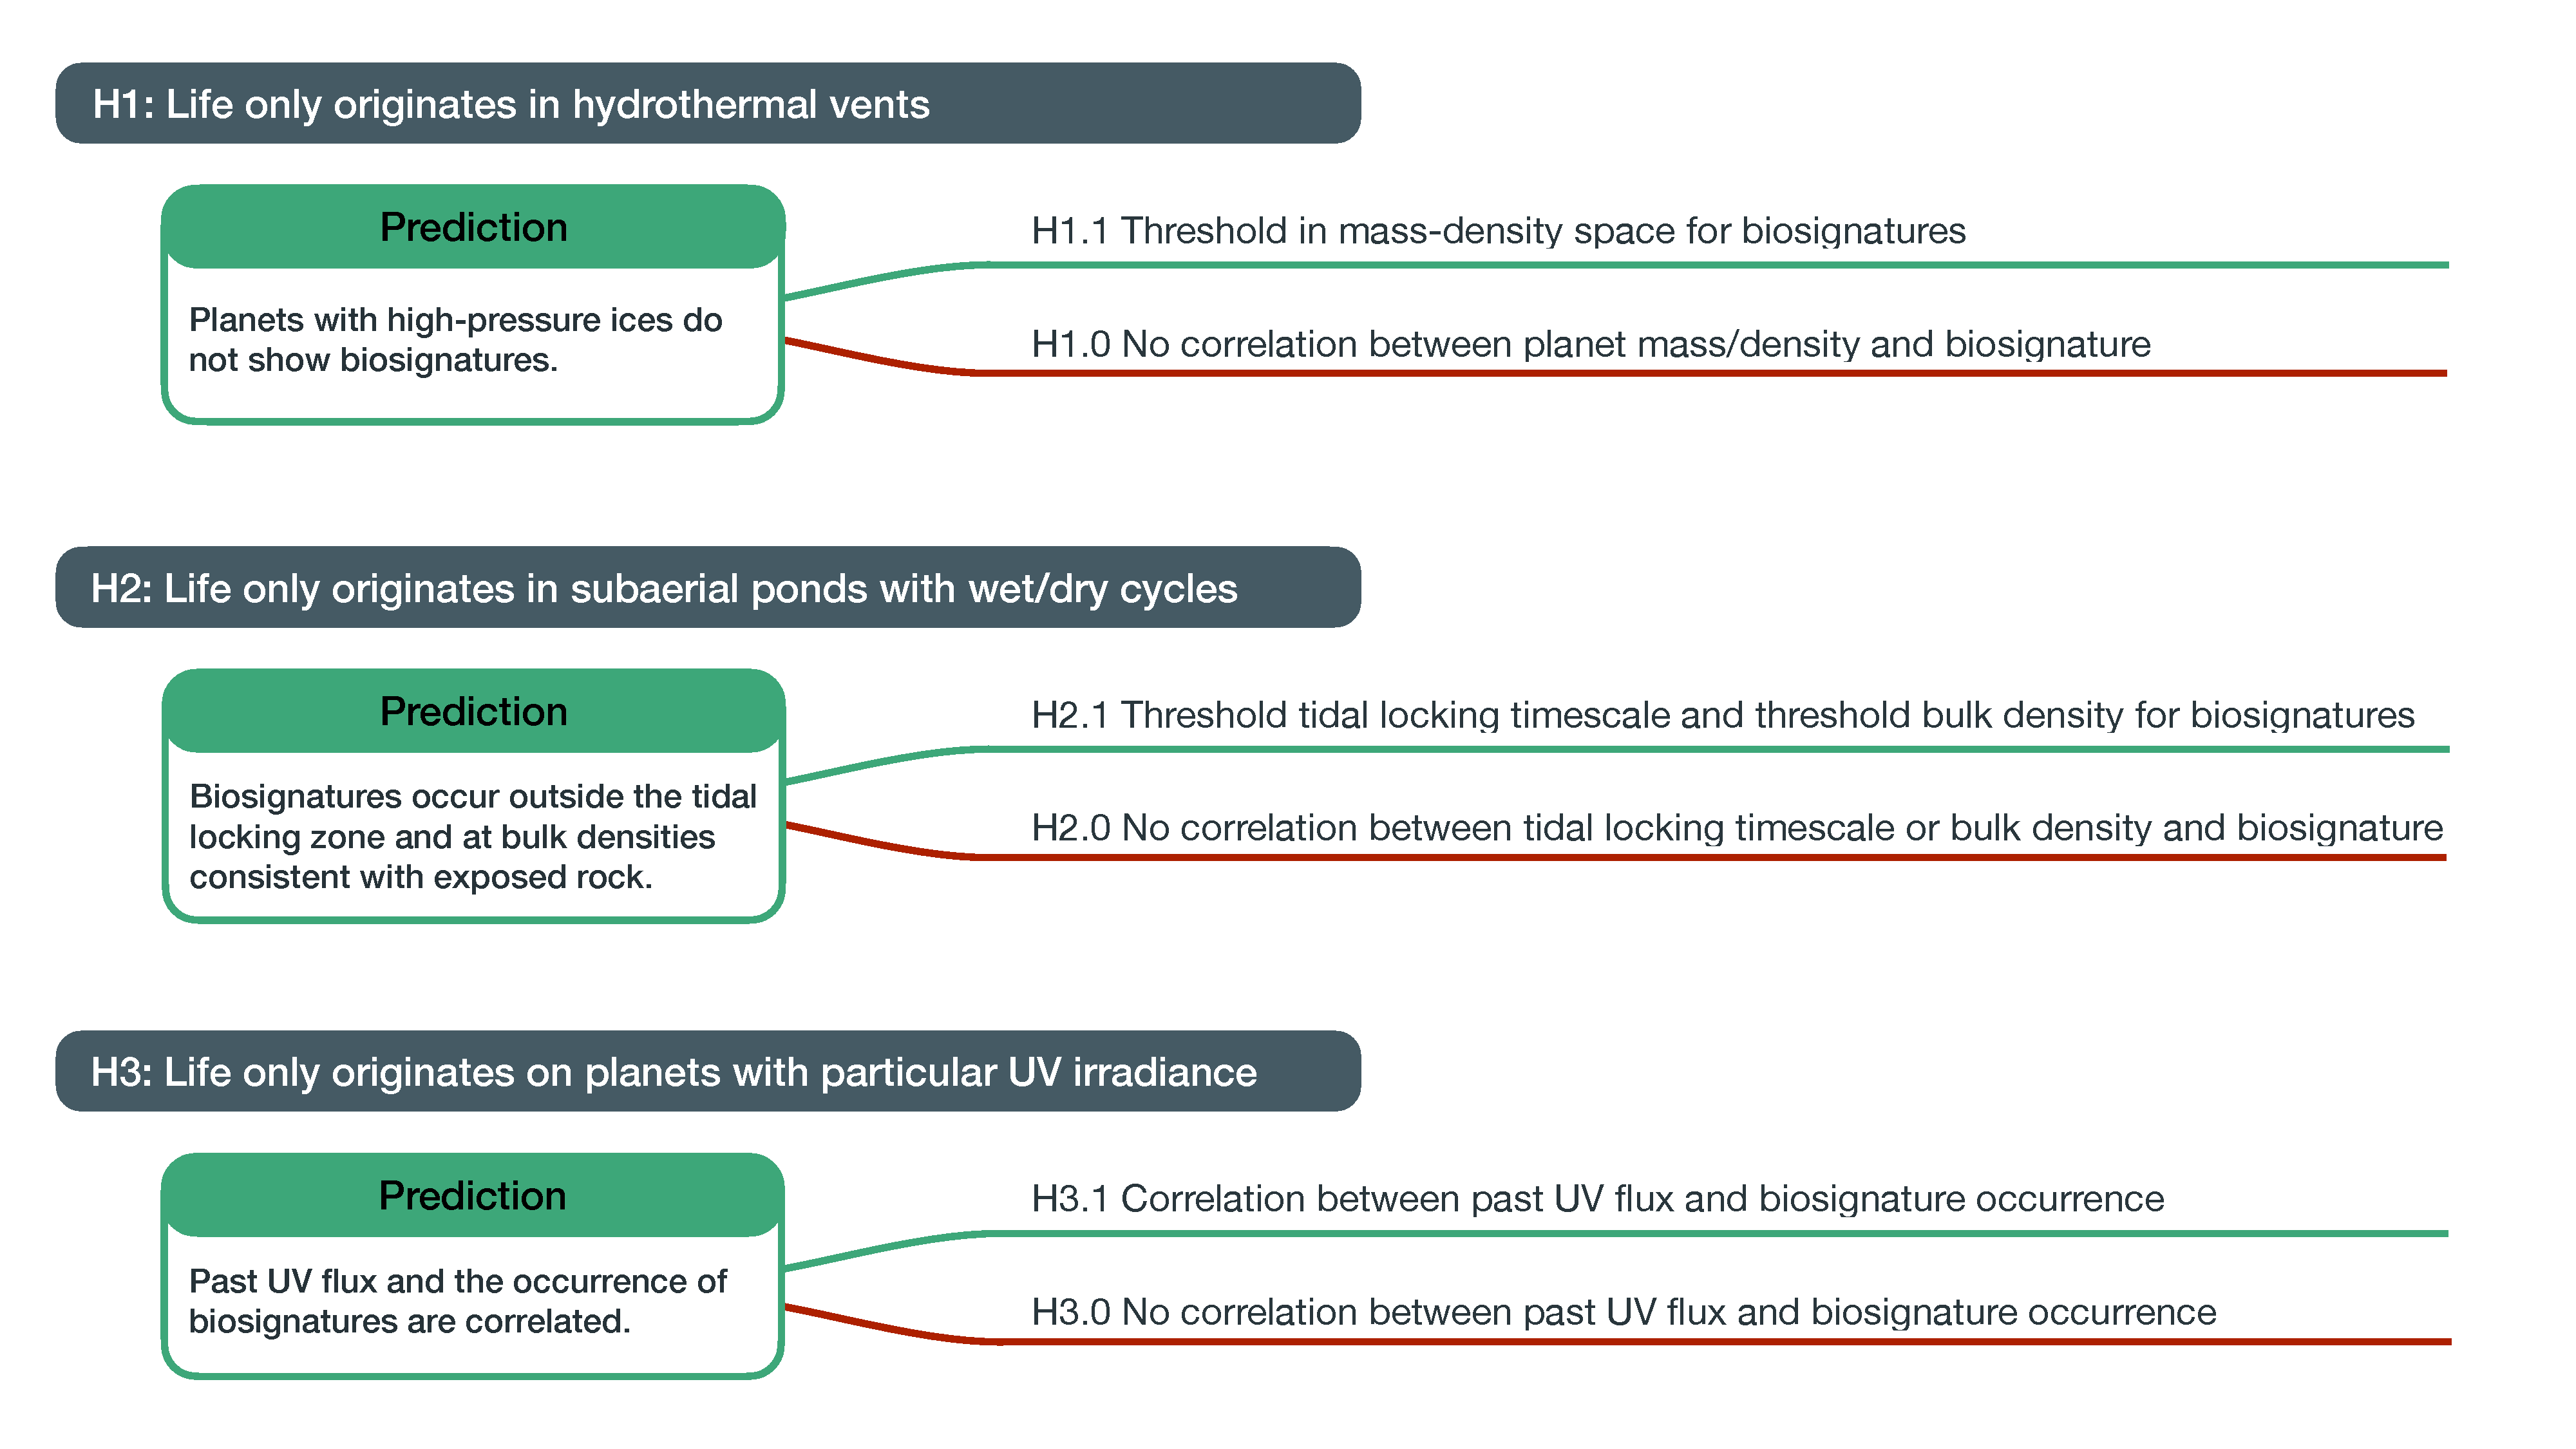
\includegraphics[width=\hsize]{figures/hypotheses}
        \caption{Population-level hypothesis and null hypothesis on UV irradiance derived from the cyanosulfidic scenario.}
        \label{fig:hypotheses}
    \end{centering}
\end{figure*}
Figure~\ref{fig:hypotheses} shows the hypothesis and null hypothesis derived from the predictions of the cyanosulfidic scenario.
...


\section{Methods}
\label{sec:hypotests}
\todo[inline]{Briefly introduce Bayesian model comparison, then present the particular hypotheses in their mathematical form.}


\subsection{Fraction of inhabited planets with detectable biosignatures}
Presumably, not all habitable worlds are inhabited and not all inhabited worlds develop detectable biosignatures.
The fraction of \glspl{EEC} that are both inhabited and harbor detectable biosignatures at the time when we observe them remains speculative; we aggregate them in the unitless parameter $f_\mathrm{life}$.

%\subsection{H1: Life only originates in hydrothermal vents}
%The hydrothermal vent scenario does not allow oceans deep enough to form an impenetrable layer of high-pressure ice on its floor.
%The resulting allowed parameter space is described by a lower limit on the bulk density. \todo[inline]{+ exclude atmospheric signature for water worlds?}
%...
%
%\subsection{H2: Life only originates in subaerial ponds with wet/dry cycles}
%We parametrize the required exposed land surface in this scenario as a lower limit in bulk density that is higher than for H1.
%Further, the tidal locking timescale of the planet may not be smaller than the age of the system.
%...
%
%\subsection{H3: Life only originates on planets with particular UV irradiance}
\todo[inline]{\citet{Guenther2020} relate U-band energy to bolometric flux.}
\todo[inline]{OPTIONAL: ``We further test the scenario of a linear correlation of past UV flux and biosignature occurrence rate.
This test requires the detection of multiple biosignatures.''
~\\
Test for negative correlations as well?}
Our third theoretical experiment is to test the UV irradiance requirement (Sect.~\ref{sec:predictions}) by relating the occurrence of life on an exo-earth candidate with a minimum past quiescent stellar UV flux, focusing on the prebiotically interesting \gls{NUV} range from \SIrange{200}{280}{\nano\meter}. \todo[inline]{SUKRIT: got a good reference for this?}  %~\citep{RanjanSasselov2016}.?
Our concrete hypothesis shall be that life only occurs on planets that at some point in their history have received such radiation exceeded a minimum flux $F_\mathrm{NUV, min}$.



\subsection{Semi-analytical analysis}\label{sec:met-semianalytical}
First, we apply a Bayes Factor Design Analysis~\citep{Schoenbrodt2018} to assess the expected probabilities of obtaining true negative or true positive evidence for the hypothesis above, as well as the probability for misleading or inconclusive evidence.

Let our observable be the inferred past \gls{NUV} flux of the planet $F_\mathrm{NUV}$.
Under Hypothesis $H_1$ (Equation~\ref{eq:hypothesis-uv}), there exists a special unknown value of $F_\mathrm{NUV}$, noted $F_\mathrm{NUV, min}$ such that

\begin{align}
    P(L|\theta,H_1) &=  f_\mathrm{life} \quad \text{if } \theta>F_\mathrm{NUV, min}\\
    P(L|\theta,H_1) &=  0               \quad  \text{otherwise}
\end{align}

where $f_\mathrm{life}$ is the unknown probability of abiogenesis.
The corresponding null hypothesis is that there exists no such special value of $F_\mathrm{NUV}$ and that
\begin{equation}
P(L|\theta,H_\mathrm{null}) = f_\mathrm{life}.
\end{equation}

If we now define a sample of size $n$ as $X=\{F_\mathrm{NUV, i},L_i\}_{i \in [1,n]}$ where $L_i$ is equal to 1 if life is detected and 0 otherwise, we can calculate the evidence for hypothesis $H_i$ against $H_j$ through the Bayes factor
\begin{equation}
BF_{H_i,H_j} = \frac{P(X|H_i)}{P(X|H_j)},
\end{equation}
with $P(X|H_i)$ and $P(X|H_j)$ likelihoods of obtaining the sample $X$ under either hypothesis.

If we define $k=\sum L_i$ and denote $Y$ the random variable that describes it, $H_\mathrm{null}$ represents the likelihood that the number of planets with life in the sample follows the binomial distribution
\begin{equation}
P(Y=k|H_\mathrm{null}) = \binom{n}{k}f_\mathrm{life}^k(1-f_\mathrm{life})^{n-k}.
\end{equation}

Under $H_1$, $Y$ also follows a binomial distribution, however it is conditioned by $n_{\lambda}=Card(\{F_\mathrm{NUV, i} \text{ if } F_\mathrm{NUV, i}>F_\mathrm{NUV, min}\}_{i \in [1,n]})$ the number of values of $F_\mathrm{NUV}$ in the experiment that exceed $F_\mathrm{NUV, min}$
\begin{equation}
P(Y=k|H_1) = \binom{n_{\lambda}}{k}f_\mathrm{life}^k(1-f_\mathrm{life})^{n_{\lambda}-k}.
\end{equation}

Hence,
\begin{equation}\label{eq:bayes_factor}
BF_{H_1,H_\mathrm{null}} = \frac{P(Y=k|H_1)}{P(Y=k|H_\mathrm{null})} = \frac{\binom{n_\lambda}{k}}{\binom{n}{k}}(1-f_\mathrm{life})^{n_{\lambda}-n}.
\end{equation}


Given a sample of planets, where for some of them we have convincing biosignature detections but remaining agnostic on $f_\mathrm{life}$: What evidence for $H_\mathrm{1}$ and $H_\mathrm{null}$ can we expect to get?
Our Bayes factor (Equation~\ref{eq:bayes_factor}) is determined by the unknown variables $f_\mathrm{life}$ and $F_\mathrm{NUV, min}$, as well as the number of planets with biosignature detections in the sample $k$.
To compute the distribution of evidences, we repeatedly generated samples under $H_\mathrm{1}$ and $H_\mathrm{null}$ and computed the Bayes factors $BF_{H_1,H_\mathrm{null}}$ and $BF_{H_\mathrm{null}, H_1}$.
We then evaluated the fraction of Monte Carlo runs in which certain evidence thresholds~\citep{Jeffreys1939} were exceeded.


%\subsection{Bayesian hypothesis testing with \bioverse}

\subsection{Considered planets and their orbits}
All Origins of Life scenarios considered here require water as a solvent; we thus consider only rocky planets that may sustain liquid water on their surface.
Different formulations of habitable zones as regions around a star where a planet with Earth's atmospheric composition can maintain liquid water on its surface exist~\citep[e.g.,][]{MolLous2022,Spinelli2023,Tuchow2023}. CITE! Ramirez \& Kaltenegger 2017, 2018
Here, we adopt the popular estimates of \citet{Kasting1993} and \citet{Kopparapu2013,Kopparapu2014} that define a temperate zone between the runaway greenhouse transition CITE! and the maximum greenhouse limit CITE!.
We use the parametrization in \citet{Kopparapu2014} to derive luminosity and planetary mass-dependent edges of the \gls{HZ} $a_\mathrm{inner}$ and $a_\mathrm{outer}$.
We further follow \citet{Bixel2021} and classify as \glspl{EEC} all planets with radii $0.8 S^{0.25} < R < 1.4 $ that orbit within the above boundaries.
The lower limit was suggested as a minimum planet size to retain an atmosphere~\citep{Zahnle2017}.


\todo[inline]{biosignatures: Focus on molecular Oxygen? Excess Methane? \citep[e.g.,][]{Seeburger2023}}
% detecting methanogenic life: Sandora2020, Wang2018,
A commonly discussed biosignature is molecular Oxygen (O$_2$), which on Earth emerged as a byproduct of photosynthesis during the Proterozoic era.
No individual component of an atmosphere has been identified as a reliable biosignature in isolation~\citep{Seager2016}, and the detection of Oxygen alone will certainly not be sufficient to confirm the presence of life.
Nevertheless, we focus here on detecting this key absorber as it represents the general inherent observational challenges and trends.







\subsection{Exoplanet survey simulations with Bioverse}
To model the sensitivity of the information gain of a proposed mission to sample selection and survey strategy, we now conduct survey simulations with Bioverse using different sample sizes and survey strategies.
We again require that life occurs only on planets with sufficient past UV irradiation exceeding $F_\mathrm{NUV, min}$.
Further, we require this flux to have lasted for a minimum duration $\Delta T_\mathrm{min}$ to allow for a sufficient ``origins timescale''~\citep{Rimmer2023}, and the planet to be within its momentary \gls{HZ} during this entire period.

To determine \gls{HZ} occupancy, we interpolated the stellar luminosity evolution grid of \citet{Baraffe1998} using a Clough Tocher interpolant~\citep[][see left panel of Figure~\ref{fig:hz_nuv_evo}]{Nielson1983,Alfeld1984} to compute the evolution of the inner (runaway greenhouse) and outer (maximum greenhouse) edges as a function of planet mass and stellar spectral type~\citep{Kopparapu2014}.
This provides each planet's epochs within and outside the \gls{HZ}.
For the \gls{NUV} flux, we use the age- and stellar mass-dependent \gls{NUV} fluxes in the \gls{HZ} obtained by \citet{Richey-Yowell2023}.
We linearly interpolate in their measured grid, where we convert spectral type to stellar mass using the midpoints of their mass ranges (\SI{0.75}{\Msun} for K~stars, \SI{0.475}{\Msun} for early-type M~stars,  and \SI{0.215}{\Msun} for late-type M~stars).
Outside of the age and stellar mass range covered in \citet{Richey-Yowell2023}, we extrapolate using nearest simplex (see right panel of Figure~\ref{fig:hz_nuv_evo}).

We then determined which planets were both in the \gls{HZ} and had \gls{NUV} fluxes above $F_\mathrm{NUV, min}$ for $\Delta T_\mathrm{min} \geq \var{deltaT_min}\,\SI{}{\mega\year}$.
We assigned the development of life to a random fraction $f_\mathrm{life}$ of all temperate planets fulfilling these requirements.
For a population-level hypothesis, we then have
\begin{equation}\label{eq:hypothesis-uv}
    H_{1} = f_\mathrm{life} (\theta, F_\mathrm{NUV}) =
        \begin{cases}
            0 , & F_\mathrm{NUV} < F_\mathrm{NUV, min}\\
            f_\mathrm{life}, & F_\mathrm{NUV} \geq F_\mathrm{NUV, min} \,\mathrm{and\, in\, HZ} \, \mathrm{for} \, \Delta t \geq \var{deltaT_min} \,\SI{}{\mega\year}
        \end{cases}
\end{equation}
and the corresponding null hypothesis
%\begin{equation}
$H_{null} = f_\mathrm{life} (\theta),$
%\end{equation}
i.e., no correlation with UV flux.



\begin{figure}
    \script{inhabited_FGKM.py}
    \begin{centering}
        \includegraphics[width=\hsize]{figures/inhabited_FGKM}
        \caption{Host stars of all transiting planets, \glspl{EEC}, and inhabited planets. In a sample of \var{N_nautilus} transiting planets, most \glspl{EEC} and all inhabited planets orbit M~dwarfs.}
        \label{fig:inhabited_FGKM}
    \end{centering}
\end{figure}

As shown in Figure~\ref{fig:inhabited_FGKM}, the majority of \glspl{EEC} and all inhabited planets orbit M~dwarfs.


\begin{figure*}
    \script{hz_nuv_evo.py}
    \begin{centering}
        \includegraphics[width=\hsize]{figures/hz_nuv_evo}
        \caption{Interpolated stellar luminosity evolution (left) and evolution of the \gls{NUV} flux in the \gls{HZ} as a function of host star mass. The scatter plot shows age and host star mass of the transiting planets in the synthetic sample.% with \gls{EEC} highlighted in green.
        We show the evolutionary tracks of a few randomly selected planets.
        Tracks with extended overlap of \gls{HZ} occupancy and high \gls{NUV} flux (green sections) fulfill our requirement for abiogenesis.}
        \label{fig:hz_nuv_evo}
    \end{centering}
\end{figure*}




\subsubsection{Transit survey (e.g., Nautilus)}

\subsubsection{Direct imaging survey (e.g., Habitable Worlds Observatory, LIFE)}
%\subsubsubsection{target list}
%\todo[inline]{Provisional stellar target List for the habitable Worlds Observatory:~\citep{Mamajek2023}} % read like in https://github.com/mkenworthy/HWObows/tree/40b1e5f2bc2bbbe8c999b097c80ca5a8cda0aeae/src/scripts







\section{Results}
\label{sec:results}
%\subsection{Information content in mass-density space}
%\subsection{Information content in tidal locking timescale-density space}

%\subsection{Correlation of past UV flux and biosignature occurrence}\label{sec:results_uv}

\subsection{Semi-analytical approach}
In Section~\ref{sec:met-semianalytical} we computed the probability for true positive evidence for $H_\mathrm{1}$ and $H_\mathrm{null}$ respectively.
Figure~\ref{fig:semian_true_evidence} shows how these evidences are distributed for sample sizes \var{semian_Nsamp1} and \var{semian_Nsamp2}, and how likely we are to obtain strong evidence ($BF_{H_i, H_j}$ > 10).
For $n = \var{semian_Nsamp1}$, strong true evidence for $H_\mathrm{1}$ ($H_\mathrm{null}$) can be expected in $\sim \SI{30}{\percent}$ ($\sim \SI{40}{\percent}$) of all random experiments.
In the majority of cases, the outcome of the survey will be inconclusive.
\begin{figure*}
    \script{semian_true_evidence.py}
    \begin{centering}
        \includegraphics[width=\hsize]{figures/semian_true_evidence}
        \caption{Probability to obtain true strong evidence. Left: evidence levels for $H_\mathrm{1}$ and $H_\mathrm{null}$ under sample sizes $n = \var{semian_Nsamp1}$ (solid) and $n = \var{semian_Nsamp2}$ (dashed). The vertical lines denote the thresholds for ``strong'' evidence, $BF_{H_i, H_j}$ > 10, and ``extreme'' evidence, $BF_{H_i, H_j}$ > 100. Right: Probability of true strong evidence for $H_\mathrm{1}$ or $H_\mathrm{null}$, whichever is smaller, as a function of sample size $n$.}
        \label{fig:semian_true_evidence}
    \end{centering}
\end{figure*}
The situation improves with larger samples: for $n = \var{semian_Nsamp2}$, \SI{80}{\percent} of random experiments yield true strong evidence under either $H_\mathrm{1}$ or $H_\mathrm{null}$.

The expected resulting evidence further depends on the a priori unknown abiogenesis rate $f_\mathrm{life}$ and on the \gls{NUV} flux threshold.
\begin{figure*}
    \script{semian_true_evidence.py}
    \begin{centering}
        \includegraphics[width=\hsize]{figures/semian_evidence-grid}
        \caption{Probability of obtaining true strong evidence for different abiogenesis rates, \gls{NUV} flux thresholds, and sample sizes. For each of these parameters, higher values increase the probability of yielding strong evidence.}
        \label{fig:semian_evidence-grid}
    \end{centering}
\end{figure*}
Figure~\ref{fig:semian_evidence-grid} illustrates this dependency: For very low values of either parameter, samples drawn under the null or alternative hypotheses are indistinguishable and the Bayesian evidence is always low.
Both higher $f_\mathrm{life}$ and higher \gls{NUV} flux thresholds increase the probability of obtaining strong evidence.
Larger sample sizes enable this at lower values of these parameters.


So far, we have assumed random, uniform distributions of $f_\mathrm{life}$, $F_\mathrm{NUV, min}$, and $F_\mathrm{NUV}$.
A high biosignature detection rate $f_\mathrm{life}$ increases the evidence (cmp. Equation~\ref{eq:bayes_factor}) but we cannot influence it.
The same is true for $F_\mathrm{NUV, min}$, where again higher values increase the evidence as the binomial distribution for $H_\mathrm{1}$ gets increasingly skewed and shifted away from the one for $H_\mathrm{null}$.
The distribution of $F_\mathrm{NUV}$ in the planet sample, on the other hand, can be influenced by the survey strategy.
A targeted sampling approach could be to favor extreme values of $F_\mathrm{NUV}$ in the sample selection.
Figure~\ref{fig:semian_selectivity} shows how the probability of obtaining true strong evidence for $H_\mathrm{1}$ scales with selectivity $s$, where $s\in]-1,1[$ such that $F_\mathrm{NUV} \sim Beta(1/10^s,1/10^s)$.
Here, $s=0$ corresponds to a random uniform distribution.
Compared to this case, a high selectivity can increase the probability of obtaining true strong evidence to $\gtrsim \SI{85}{\percent}$ for large samples.

\begin{figure}
    \script{semian_true_evidence.py}
    \begin{centering}
        \includegraphics[width=\hsize]{figures/semian_selectivity}
        \caption{Scaling of the probability of obtaining true strong evidence with sample selectivity. Left: Sampling distribution for different selectivity parameters $s$. Right: Resulting \mbox{P(true strong evidence)} (random, uniform $f_\mathrm{life}$, $F_\mathrm{NUV, min}$). Sampling more extreme values of $F_\mathrm{NUV}$ is more likely to yield strong evidence.}
        \label{fig:semian_selectivity}
    \end{centering}
\end{figure}




\subsection{Survey simulations with Bioverse}

In a magnitude- and volume-limited sample of a transit survey, the host star distribution will be skewed toward later spectral types and dominated by M~dwarfs (see Figure~\ref{fig:inhabited_FGKM}).
Due to how the \gls{HZ} scales with spectral type, by far most transiting \glspl{EEC} occur around M~dwarfs.
These host stars, in particular late subtypes, also provide extended periods of increased \gls{NUV} emission that overlap with times when some of these planets occupy the \gls{HZ} (see Figure~\ref{fig:hz_nuv_evo}), our requirement for abiogenesis (compare Equation~\ref{eq:hypothesis-uv}).
Because of that, all inhabited planets orbit M~dwarfs.


A representative recovery of the injected biosignature pattern is shown in Figure~\ref{fig:detections_uv}.
There, we assumed an abiogenesis rate of $f_\mathrm{life} = \var{f_life}$ and a minimum \gls{NUV} flux of $F_\mathrm{NUV, min} = \var{NUV_thresh}\,\SI{}{\photons\per\centi\meter\squared\per\second\per\nano\meter}$.
This leads to a distribution of biosignature detections with detections increasingly occurring above a threshold inferred NUV flux.
\begin{figure}
    \script{detections_uv.py}
    \begin{centering}
        \includegraphics[width=\hsize]{figures/detections_uv}
        \caption{Recovered biosignature detections in the \gls{NUV} flux -- biosignature occurrence space. The dashed line denotes the threshold \gls{NUV} flux $F_\mathrm{NUV, min}$.}
        \label{fig:detections_uv}
    \end{centering}
\end{figure}


We now investigate the sensitivity of the achieved statistical power of our default transit survey to the a priori unconstrained threshold \gls{NUV} flux $F_\mathrm{NUV, min}$ and the abiogenesis rate $f_\mathrm{life}$.
Figure~\ref{fig:powergrid} shows the statistical power as a function of these parameters for a sample size of $N=\var{N_nautilus}$.
Values of $F_\mathrm{NUV, min}$ that lie between the extrema of the inferred maximum \gls{NUV} flux increase the achieved statistical power of the survey, as in this case the dataset under the alternative hypothesis $H_1$ differs more from the null hypothesis.
The same is true for the abiogenesis rate $f_\mathrm{life}$, where higher values increase the evidence for $H_1$.

\begin{figure}
    \script{powergrid.py}
    \begin{centering}
        \includegraphics[width=\hsize]{figures/powergrid}
        \caption{Statistical power as a function of threshold \gls{NUV} flux and abiogenesis rate. For a given sample size (here: $N=\var{N_nautilus}$), the achieved statistical power of the survey is enhanced for higher values of $f_\mathrm{life}$ and intermediate values of $F_\mathrm{NUV, min}$.}
        \label{fig:powergrid}
    \end{centering}
\end{figure}



\section{Discussion}
\label{sec:discussion}
%''Which natural processes best explain how living matter spontaneously appears from nonliving matter?''~\citep{Malaterre2022}
%WE consider life ``as we know it''

\subsection{What do we learn from a single biosignature detection?}
\todo[inline]{discuss constraining power on OOL of a convincing biosignature detection on a single planet, depending on the position of the planet in the parameter space we explored.}

\subsection{Constraining power for the origins of life as a function of biosignature location}
\todo[inline]{How does the location of biosignature detections impact the credibility of OOL scenarios?}
\todo[inline]{biosignature on M~dwarf planet vs. FGK: Impact on UV flux requirement?}
\subsubsection{Sampling strategy for testing a predicted minimum \gls{NUV} flux}
We show in Sect.~\ref{sec:results} that the constraining power for testing the hypothesis of a minimum past \gls{NUV} flux required for abiogenesis is sensitive on the occurrence of life, the value of this threshold flux, the sample size, and the distribution of sampled past \gls{NUV} fluxes.
In particular the last parameter offers an opportunity to optimize the survey strategy: Although constraints on a planet's UV history have generally large uncertainties~\citep[e.g.,][]{Richey-Yowell2023}, the likely maximum flux of a planet can be inferred and used as a proxy.
Sampling more extreme (low and high) values for the maximum flux increases the probability of obtaining true strong evidence for the hypothesis.
For large sample sizes $\gtrsim 200$, this strategy can push this probability into the \SI{90}{\percent} range.
\todo[inline]{and what about the probability of getting true strong evidence for H0?}




\subsection{Contextual support for potential biosignature detections}
\todo[inline]{discuss how planetary context may impact credibility of tentative biosignature detections (e.g., if there is a good fit with a predicted OOL pattern; or the opposite: the planetary context does not fit well to any OOL scenarios)}
As we have shown in Section~\ref{sec:results}, the interplay of \gls{NUV} evolution and \gls{HZ} occupancy strongly favors late spectral types for abiogenesis via the cyanosulfidic scenario.
This strong predicted correlation between stellar spectral type and the occurrence of life can be used to falsify \gls{ool} scenarios.
The constraint of this context is particularly strong if a candidate biosignature is detected on a planet orbiting an earlier type star, i.e., where it is unexpected in the context of this \gls{ool} scenario.



\subsection{Caveats}
\subsubsection{Atmosphere transmission}
Theoretical work suggests that the atmosphere of prebiotic Earth was largely transparent at near-UV wavelengths with the only known source of attenuation being Rayleigh scattering~\citep{Ranjan2017,Ranjan2017c}.
We thus approximated surface UV flux using top-of-atmosphere fluxes.
This represents a conservative approach, since any planet that fails to meet the irradiance criterion receives even lower near-UV radiation at its surface. \todo[inline]{SUKRIT please specify as neccessary}

\subsubsection{Stellar flares}
Our assumptions on past UV flux neglect the contribution of stellar flares, which may be hypothesized as an alternative source of UV light~\citep{Ranjan2017}.
This concerns mainly ultracool dwarfs, due to their low quiescent emission and high pre-main sequence stellar activity~\citep{Buccino2007,West2008}.
Recent work indicates that the majority of stars show inadequate activity levels for a sufficient contribution through flares~\citep{Glazier2020,Ducrot2020,Guenther2020}.
The biosignature surveys we simulated here may test the hypothesis of sufficient UV radiation via stellar flares.

%\subsubsection{Diurnal cycles}
%\todo[inline]{We assume that tidal locking implies that there are no wet-dry cycles. Challenge this assumption.}


\section{Conclusions and future work}

Our main findings are:
\begin{enumerate}
    \item Models of the Origins of Life provide hypotheses that are testable with near-future exoplanet surveys.
    \item The required \gls{NUV} radiation in the cyanosulfidic scenario should lead to a correlation between past \gls{NUV} flux and current occurrence of biosignatures, both of which will soon be observationally accessible.
    \item The required sample size for detecting this correlation depends on the occurrence of life on temperate exoplanets, the distribution of host star spectral types in the sample, ...
        A direct imaging mission with the \gls{HWO} will require characterizing XXX planets ...
    \item If the predicted \gls{NUV} correlation exists, yielding strong evidence for it is likely ($> \SI{90}{\percent}$) for sample sizes $\geq 100$, and a survey strategy that targets extreme values of inferred past \gls{NUV} irradiation.
    \item Abiogenesis in the cyanosulfidic scenario strongly prefers late host star spectral types in a sample of transiting planets. Any potential biosignature detection on a planet around a star other than an M~dwarf would disvafor this scenario and any other \gls{ool} theory requiring extended periods of high \gls{NUV} irradiation.
\end{enumerate}

%\begin{acknowledgments}
\section*{Acknowledgments}
    The authors thank Kevin Heng, Dominik Hintz, Chia-Lung Lin, and Rhys Seeburger for insightful discussions.
%    We are grateful to ...
%    mention any people who gave comments in early-on meetings
    We thank the anonymous referee for providing constructive critical feedback that helped to improve this manuscript.
    This material is based upon work supported by the National Aeronautics and Space Administration under Agreement No. 80NSSC21K0593 for the program ``Alien Earths''.
    The results reported herein benefited from collaborations and/or information exchange within NASA’s Nexus for Exoplanet System Science (NExSS) research coordination network sponsored by NASA’s Science Mission Directorate.
    This work has made use of data from the European Space Agency (ESA) mission \gaia\ (\url{https://www.cosmos.esa.int/gaia}), processed by the \gaia\ Data Processing and Analysis Consortium (DPAC, \url{https://www.cosmos.esa.int/web/gaia/dpac/consortium}). Funding for the DPAC has been provided by national institutions, in particular the institutions participating in the \gaia\ Multilateral Agreement.
    T.L. was supported by the Branco Weiss Foundation, the Netherlands eScience Center (PROTEUS project, NLESC.OEC.2023.017), and the Alfred P. Sloan Foundation (AEThER project, G202114194).
%    ...
\end{acknowledgments}

\section*{Author contributions}
M.S., D.A., and S.R.\ conceived the project, planned its implementation, and interpreted the results.
M.S.\ developed the planetary evolution component to \bioverse, carried out the hypothesis tests and statistical analyses, and wrote the manuscript.
D.A.\ leads the ``Alien Earths'' program through which this project is funded, helped to guide the strategy of the project, and provided text contributions.
A.A.\ carried out the semi-analytical computations regarding the correlation of past UV flux and biosignature occurrence.
S.R.\ advised on planetary \gls{NUV} flux evolution and the cyanosulfidic scenario of the origins of life.
R.F.\ wrote the initial draft of the Introduction and advised on the evolutionary biology aspects of the project.
K.H.-U.\ contributed to the \bioverse\ software development and simulations.
%M.S.\ wrote the manuscript; ... and ... provided text contributions.
T.L.\ supported the selection of testable hypotheses and provided text contributions to the initial draft.
S.M.\ advised on the scope of the project and supported the selection of testable hypotheses.
All authors provided comments and suggestions on the manuscript.


%Author affiliations (tbd):
%Martin Schlecker1, Daniel Apai1,2, Antonin Affholder4, Sukrit Ranjan2, Regis Ferriere4, Kevin Hardegree-Ullman1, Tim Lichtenberg3, and Stephane Mazevet5
%1 Steward Observatory and Department of Astronomy, The University of Arizona, Tucson, AZ 85721, USA
%2 Lunar and Planetary Laboratory, The University of Arizona, Tucson, AZ 85721, USA
%3 Kapteyn Astronomical Institute, University of Groningen, PO Box 800, 9700 AV Groningen, The Netherlands
%4 Department of Ecology and Evolutionary Biology, University of Arizona, Tucson, AZ, USA
%5 Observatoire de la Côte d’Azur, 96 Boulevard de l’Observatoire, F-06300 Nice, France


\section*{Reproducibility}

%! suppress = MissingBibliographystyle
\bibliography{bib,coauthors}

\end{document}
